\chapter{CONCLUSÃO}
\label{chap:conclusao}

\par A partir das discussões propostas por este trabalho e dos resultados obtidos é possível afirmar que o método de extração de características com árvore geradora mínima se mostra eficaz e pode ser utilizado para a caracterização de texturas de imagens.

\par Ao observar o \textit{dataset} USC-SIPI \textit{Textures}, pode-se concluir que o extrator proposto, MST, obteve resultados tão bons quanto os extratores comparados, sendo capaz até mesmo de supera-los quando utilizado com SVC. Com o \textit{dataset} de Kylberg, os resultados não foram muito diferentes, apesar do extrator LBP se manter como melhor em todos os cenários, o extrator proposto se mantém em segundo lugar em quase todos os testes. Porém, o MST não apresentou resultados animadores durante os testes com o \textit{dataset} USPtex, exceto pelo extrator LBP, os outros também não apresentaram resultados significantes. Por fim, para o \textit{dataset} VisTex, nenhum extrator obteve uma acurácia maior que 55\% em todos os tipos testes, sendo o extrator proposto mantido em segundo lugar e em primeiro quando utilizado com \textit{Decision Tree}. Mais informações sobre os resultados estão disponíveis no \textit{github}\footnote{\url{https://github.com/felipeseolin/image-texture-classification-tests}}, assim com o código fonte do extrator\footnote{\url{https://github.com/felipeseolin/image-texture-classification}}.

\par Apesar de existirem casos em que outros algoritmos obtiveram melhores resultados de acurácia e matriz de confusão, o extrator proposto foi capaz de coletar com eficácia as informações necessárias para o reconhecimento texturas de imagens com um número reduzido de características. A \autoref{tab:extratorXqtdCaracteristicas}, apresenta a relação entre os extratores e número de características que cada um deles utiliza.

\begin{table}[H]
    \centering
    \caption[Extratores e quantidades de características]{Extratores e quantidades de características
    \label{tab:extratorXqtdCaracteristicas}}
    \begin{tabular}{cc}
        \toprule
            Extrator & Números de características \\
        \midrule
            Gabor & 60 \\
            Haralick & 14 \\
            LBP & 256 \\
            Tamura & 18 \\
            MST & 5 \\
        \bottomrule
    \end{tabular}
    \fonte{Autoria Própria.}
\end{table}


% \par (REVER) É importante destacar que medidas de custo computacional e tempo de execução não foram levadas em consideração neste trabalho, pois o processo de extração de características de uma imagem (descrição) é, em geral, um processo custoso e demorado, sendo sempre realizado de forma prévia.
% \par No entanto, é importante ressaltar que o algoritmo proposto apresentou um tempo relativamente alto, quando comparado aos outros algoritmos, o que faz com que ele precise ser aperfeiçoado e otimizado. Isto pode ser feito reduzindo o uso de algumas bibliotecas que fornecem objetos e funções não necessárias, mas mesmo assim o processamento é executado. Como exemplo, a biblioteca igraph a qual retorna sempre um objeto Graph como resultado, sendo que só é necessário um array com os valores das arestas da MST.

\par Com o intuito de fornecer maiores comparações com os extratores e estabelecer melhores métricas, foram realizados testes sobre o tempo de execução com a \autoref{fig:tempoExecucao} retirada do \textit{dataset} USC-SIPI \textit{Textures}. Vale ressaltar que o computador utilizado possui processador Intel Core i5-8250U, CPU 1.60GHz 1.80GHz, 8GB de memória RAM instalada e 7.90GB utilizável, além de com o sistema operacional Windows 11 arquitetura \textit{64-bits}.

\pagebreak 

\begin{figure}[!h]
    \centering
    \caption{Imagem utilizada para calcular o tempo de execução.}
    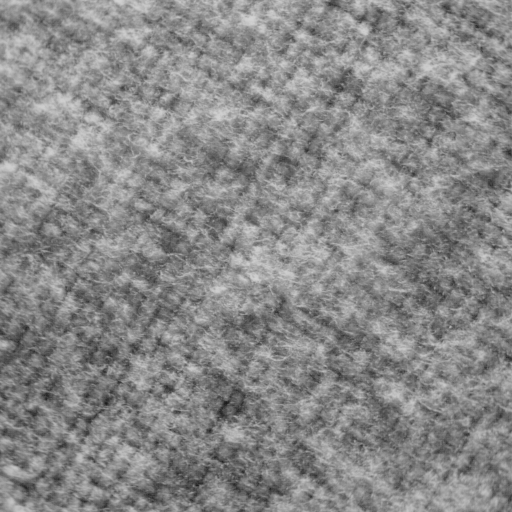
\includegraphics[width=0.5\textwidth]{./dados/figuras/testeExecucao.png}
    \fonte{\citeonline{weber1997usc}}
    \label{fig:tempoExecucao}
\end{figure}

\par A partir disto, na \autoref{tab:extratorXtempoExecucao} foram descritos os tempos de execução do extrator proposto em relação com os outros testados neste trabalho. Neste sentido, pode-se observar que o MST obteve um tempo de execução maior quando comparados com os outros, sendo que o extrator com o menor tempo de execução foi o Haralick. 

\begin{table}[H]
    \centering
    \caption[Extratores e tempo de execução]{Extratores e tempo de execução
    \label{tab:extratorXtempoExecucao}}
    \begin{tabular}{cc}
        \toprule
            Extrator & Tempo de execução em segundos \\
        \midrule
            Gabor & 1,13s \\
            Haralick & 1,03s \\
            LBP & 1,28s \\
            Tamura & 2,35s \\
            MST & 3,26s \\
        \bottomrule
    \end{tabular}
    \fonte{Autoria Própria.}
\end{table}


\par Dessa forma, nota-se que o extrator deve melhorar sua performe, de forma a otimizar o tempo de execução, isto seria possível reduzindo o uso de bibliotecas que podem carregar consigo funções além do necessário, como a biblioteca \textit{igraph}, a qual retorna sempre um objeto \textit{Graph} como resultado, sendo necessário apenas um \textit{array} com os valores das arestas da MST.

\par Por fim, pode-se concluir que o uso de grafos e de árvore geradora mínima, soluções já utilizadas em outros contextos de problemas na computação, mostra-se mais uma vez eficaz, agora para o reconhecimento de texturas. Além disso, vale ressaltar que nenhum descritor obteve resultados absolutamente melhores em todos os casos. Na maior parte, o algoritmo proposto se manteve como melhor, ou segundo melhor, em relação a acurácia. Estes dados provam que a criação de novos descritores é valida e necessária para o aprimoramento da área de processamento de imagens digitais.

\section{TRABALHOS FUTUROS}
\label{sec:trabalhosFuturos}

\par Em trabalhos futuros, o extrator pode ser comparado a outros extratores de textura presentes na literatura, principalmente aqueles que utilizam grafos como método principal. Também é possível mudar alguns parâmetros durante o aprendizado supervisionado, como a semente, divisão entre teste e treino, normalização e outros algoritmos.

\par Mudar a forma que os pesos das arestas são gerados e adicionar características, também poderiam aumentar a acurácia do algoritmo durante os testes, porém deve-se levar em conta o tempo de execução e custo computacional de tais mudanças. Neste sentido, a aplicação de técnicas antes mesmo do desenvolvimento do algoritmo, como a utilização de \textit{superpixels} pode reduzir o custo computacional e melhorar a performance do extrator.

\par Além disso, seria interessante aprimorar o extrator no contexto de suporte a imagens com cores RGB. Um caminho possíveis para isto é a expansão do número de ligações dos \textit{pixels}, assim um \textit{pixel} não se ligaria apenas com os \textit{pixels} de sua camada, mas também da camada inferior a este.

\par Por fim, a partir de todas as discussões levantadas por este trabalho, pode-se concluir que o desenvolvimento de diferentes trabalhos e abordagens do processamento de imagens digitais tem grande aceitação e espaço para crescimento, por isso se fazem necessárias para a evolução da área.
